\documentclass{article}

\usepackage{authblk}
% \usepackage{hyperref}
\usepackage{natbib}
\usepackage{amsthm}
\usepackage{graphicx}



%%%%% NEW MATH DEFINITIONS %%%%%

\usepackage{amsmath,amsfonts,bm}
% My personal settings
\usepackage{geometry}
\usepackage{xcolor}
\usepackage{url}
\geometry{hcentering, left=20mm, right=20mm}
\definecolor{orresBlue}{RGB}{0, 98, 158}
\usepackage[colorlinks,
            linkcolor=orresBlue,
            anchorcolor=orresBlue,
            citecolor=orresBlue
            ]{hyperref}
\renewcommand{\familydefault}{\sfdefault}

% Numbered environments and their references
\newtheorem{theorem}{Theorem}
\newtheorem{definition}{Definition}
\newtheorem{proposition}{Proposition}
\newtheorem{lemma}{Lemma}
\newtheorem{corollary}{Corollary}
\newtheorem{example}{Example}
\newtheorem{remark}{Remark}

\def\thmref#1{Theorem~\ref{#1}}
\def\defref#1{Definition~\ref{#1}}
\def\prpref#1{Proposition~\ref{#1}}
\def\lemref#1{Lemma~\ref{#1}}
\def\corref#1{Corollary~\ref{#1}}
\def\expref#1{Example~\ref{#1}}
\def\rmkref#1{Remark~\ref{#1}}

% Mark sections of captions for referring to divisions of figures
\newcommand{\figleft}{{\em (Left)}}
\newcommand{\figcenter}{{\em (Center)}}
\newcommand{\figright}{{\em (Right)}}
\newcommand{\figtop}{{\em (Top)}}
\newcommand{\figbottom}{{\em (Bottom)}}
\newcommand{\captiona}{{\em (a)}}
\newcommand{\captionb}{{\em (b)}}
\newcommand{\captionc}{{\em (c)}}
\newcommand{\captiond}{{\em (d)}}

% Highlight a newly defined term
\newcommand{\newterm}[1]{{\bf #1}}


% Figure reference, lower-case.
\def\figref#1{figure~\ref{#1}}
% Figure reference, capital. For start of sentence
\def\Figref#1{Figure~\ref{#1}}
\def\twofigref#1#2{figures \ref{#1} and \ref{#2}}
\def\quadfigref#1#2#3#4{figures \ref{#1}, \ref{#2}, \ref{#3} and \ref{#4}}
% Section reference, lower-case.
\def\secref#1{section~\ref{#1}}
% Section reference, capital.
\def\Secref#1{Section~\ref{#1}}
% Reference to two sections.
\def\twosecrefs#1#2{sections \ref{#1} and \ref{#2}}
% Reference to three sections.
\def\secrefs#1#2#3{sections \ref{#1}, \ref{#2} and \ref{#3}}
% Reference to an equation, lower-case.
\def\eqref#1{equation~\ref{#1}}
% Reference to an equation, upper case
\def\Eqref#1{Equation~\ref{#1}}
% A raw reference to an equation---avoid using if possible
\def\plaineqref#1{\ref{#1}}
% Reference to a chapter, lower-case.
\def\chapref#1{chapter~\ref{#1}}
% Reference to an equation, upper case.
\def\Chapref#1{Chapter~\ref{#1}}
% Reference to a range of chapters
\def\rangechapref#1#2{chapters\ref{#1}--\ref{#2}}
% Reference to an algorithm, lower-case.
\def\algref#1{algorithm~\ref{#1}}
% Reference to an algorithm, upper case.
\def\Algref#1{Algorithm~\ref{#1}}
\def\twoalgref#1#2{algorithms \ref{#1} and \ref{#2}}
\def\Twoalgref#1#2{Algorithms \ref{#1} and \ref{#2}}
% Reference to a part, lower case
\def\partref#1{part~\ref{#1}}
% Reference to a part, upper case
\def\Partref#1{Part~\ref{#1}}
\def\twopartref#1#2{parts \ref{#1} and \ref{#2}}

\def\ceil#1{\lceil #1 \rceil}
\def\floor#1{\lfloor #1 \rfloor}
\def\1{\bm{1}}
\newcommand{\train}{\mathcal{D}}
\newcommand{\valid}{\mathcal{D_{\mathrm{valid}}}}
\newcommand{\test}{\mathcal{D_{\mathrm{test}}}}

\def\eps{{\epsilon}}


% Random variables
\def\reta{{\textnormal{$\eta$}}}
\def\ra{{\textnormal{a}}}
\def\rb{{\textnormal{b}}}
\def\rc{{\textnormal{c}}}
\def\rd{{\textnormal{d}}}
\def\re{{\textnormal{e}}}
\def\rf{{\textnormal{f}}}
\def\rg{{\textnormal{g}}}
\def\rh{{\textnormal{h}}}
\def\ri{{\textnormal{i}}}
\def\rj{{\textnormal{j}}}
\def\rk{{\textnormal{k}}}
\def\rl{{\textnormal{l}}}
% rm is already a command, just don't name any random variables m
\def\rn{{\textnormal{n}}}
\def\ro{{\textnormal{o}}}
\def\rp{{\textnormal{p}}}
\def\rq{{\textnormal{q}}}
\def\rr{{\textnormal{r}}}
\def\rs{{\textnormal{s}}}
\def\rt{{\textnormal{t}}}
\def\ru{{\textnormal{u}}}
\def\rv{{\textnormal{v}}}
\def\rw{{\textnormal{w}}}
\def\rx{{\textnormal{x}}}
\def\ry{{\textnormal{y}}}
\def\rz{{\textnormal{z}}}

% Random vectors
\def\rvepsilon{{\mathbf{\epsilon}}}
\def\rvtheta{{\mathbf{\theta}}}
\def\rva{{\mathbf{a}}}
\def\rvb{{\mathbf{b}}}
\def\rvc{{\mathbf{c}}}
\def\rvd{{\mathbf{d}}}
\def\rve{{\mathbf{e}}}
\def\rvf{{\mathbf{f}}}
\def\rvg{{\mathbf{g}}}
\def\rvh{{\mathbf{h}}}
\def\rvu{{\mathbf{i}}}
\def\rvj{{\mathbf{j}}}
\def\rvk{{\mathbf{k}}}
\def\rvl{{\mathbf{l}}}
\def\rvm{{\mathbf{m}}}
\def\rvn{{\mathbf{n}}}
\def\rvo{{\mathbf{o}}}
\def\rvp{{\mathbf{p}}}
\def\rvq{{\mathbf{q}}}
\def\rvr{{\mathbf{r}}}
\def\rvs{{\mathbf{s}}}
\def\rvt{{\mathbf{t}}}
\def\rvu{{\mathbf{u}}}
\def\rvv{{\mathbf{v}}}
\def\rvw{{\mathbf{w}}}
\def\rvx{{\mathbf{x}}}
\def\rvy{{\mathbf{y}}}
\def\rvz{{\mathbf{z}}}

% Elements of random vectors
\def\erva{{\textnormal{a}}}
\def\ervb{{\textnormal{b}}}
\def\ervc{{\textnormal{c}}}
\def\ervd{{\textnormal{d}}}
\def\erve{{\textnormal{e}}}
\def\ervf{{\textnormal{f}}}
\def\ervg{{\textnormal{g}}}
\def\ervh{{\textnormal{h}}}
\def\ervi{{\textnormal{i}}}
\def\ervj{{\textnormal{j}}}
\def\ervk{{\textnormal{k}}}
\def\ervl{{\textnormal{l}}}
\def\ervm{{\textnormal{m}}}
\def\ervn{{\textnormal{n}}}
\def\ervo{{\textnormal{o}}}
\def\ervp{{\textnormal{p}}}
\def\ervq{{\textnormal{q}}}
\def\ervr{{\textnormal{r}}}
\def\ervs{{\textnormal{s}}}
\def\ervt{{\textnormal{t}}}
\def\ervu{{\textnormal{u}}}
\def\ervv{{\textnormal{v}}}
\def\ervw{{\textnormal{w}}}
\def\ervx{{\textnormal{x}}}
\def\ervy{{\textnormal{y}}}
\def\ervz{{\textnormal{z}}}

% Random matrices
\def\rmA{{\mathbf{A}}}
\def\rmB{{\mathbf{B}}}
\def\rmC{{\mathbf{C}}}
\def\rmD{{\mathbf{D}}}
\def\rmE{{\mathbf{E}}}
\def\rmF{{\mathbf{F}}}
\def\rmG{{\mathbf{G}}}
\def\rmH{{\mathbf{H}}}
\def\rmI{{\mathbf{I}}}
\def\rmJ{{\mathbf{J}}}
\def\rmK{{\mathbf{K}}}
\def\rmL{{\mathbf{L}}}
\def\rmM{{\mathbf{M}}}
\def\rmN{{\mathbf{N}}}
\def\rmO{{\mathbf{O}}}
\def\rmP{{\mathbf{P}}}
\def\rmQ{{\mathbf{Q}}}
\def\rmR{{\mathbf{R}}}
\def\rmS{{\mathbf{S}}}
\def\rmT{{\mathbf{T}}}
\def\rmU{{\mathbf{U}}}
\def\rmV{{\mathbf{V}}}
\def\rmW{{\mathbf{W}}}
\def\rmX{{\mathbf{X}}}
\def\rmY{{\mathbf{Y}}}
\def\rmZ{{\mathbf{Z}}}

% Elements of random matrices
\def\ermA{{\textnormal{A}}}
\def\ermB{{\textnormal{B}}}
\def\ermC{{\textnormal{C}}}
\def\ermD{{\textnormal{D}}}
\def\ermE{{\textnormal{E}}}
\def\ermF{{\textnormal{F}}}
\def\ermG{{\textnormal{G}}}
\def\ermH{{\textnormal{H}}}
\def\ermI{{\textnormal{I}}}
\def\ermJ{{\textnormal{J}}}
\def\ermK{{\textnormal{K}}}
\def\ermL{{\textnormal{L}}}
\def\ermM{{\textnormal{M}}}
\def\ermN{{\textnormal{N}}}
\def\ermO{{\textnormal{O}}}
\def\ermP{{\textnormal{P}}}
\def\ermQ{{\textnormal{Q}}}
\def\ermR{{\textnormal{R}}}
\def\ermS{{\textnormal{S}}}
\def\ermT{{\textnormal{T}}}
\def\ermU{{\textnormal{U}}}
\def\ermV{{\textnormal{V}}}
\def\ermW{{\textnormal{W}}}
\def\ermX{{\textnormal{X}}}
\def\ermY{{\textnormal{Y}}}
\def\ermZ{{\textnormal{Z}}}

% Vectors
\def\vzero{{\bm{0}}}
\def\vone{{\bm{1}}}
\def\vmu{{\bm{\mu}}}
\def\vtheta{{\bm{\theta}}}
\def\va{{\bm{a}}}
\def\vb{{\bm{b}}}
\def\vc{{\bm{c}}}
\def\vd{{\bm{d}}}
\def\ve{{\bm{e}}}
\def\vf{{\bm{f}}}
\def\vg{{\bm{g}}}
\def\vh{{\bm{h}}}
\def\vi{{\bm{i}}}
\def\vj{{\bm{j}}}
\def\vk{{\bm{k}}}
\def\vl{{\bm{l}}}
\def\vm{{\bm{m}}}
\def\vn{{\bm{n}}}
\def\vo{{\bm{o}}}
\def\vp{{\bm{p}}}
\def\vq{{\bm{q}}}
\def\vr{{\bm{r}}}
\def\vs{{\bm{s}}}
\def\vt{{\bm{t}}}
\def\vu{{\bm{u}}}
\def\vv{{\bm{v}}}
\def\vw{{\bm{w}}}
\def\vx{{\bm{x}}}
\def\vy{{\bm{y}}}
\def\vz{{\bm{z}}}

% Elements of vectors
\def\evalpha{{\alpha}}
\def\evbeta{{\beta}}
\def\evepsilon{{\epsilon}}
\def\evlambda{{\lambda}}
\def\evomega{{\omega}}
\def\evmu{{\mu}}
\def\evpsi{{\psi}}
\def\evsigma{{\sigma}}
\def\evtheta{{\theta}}
\def\eva{{a}}
\def\evb{{b}}
\def\evc{{c}}
\def\evd{{d}}
\def\eve{{e}}
\def\evf{{f}}
\def\evg{{g}}
\def\evh{{h}}
\def\evi{{i}}
\def\evj{{j}}
\def\evk{{k}}
\def\evl{{l}}
\def\evm{{m}}
\def\evn{{n}}
\def\evo{{o}}
\def\evp{{p}}
\def\evq{{q}}
\def\evr{{r}}
\def\evs{{s}}
\def\evt{{t}}
\def\evu{{u}}
\def\evv{{v}}
\def\evw{{w}}
\def\evx{{x}}
\def\evy{{y}}
\def\evz{{z}}

% Matrix
\def\mA{{\bm{A}}}
\def\mB{{\bm{B}}}
\def\mC{{\bm{C}}}
\def\mD{{\bm{D}}}
\def\mE{{\bm{E}}}
\def\mF{{\bm{F}}}
\def\mG{{\bm{G}}}
\def\mH{{\bm{H}}}
\def\mI{{\bm{I}}}
\def\mJ{{\bm{J}}}
\def\mK{{\bm{K}}}
\def\mL{{\bm{L}}}
\def\mM{{\bm{M}}}
\def\mN{{\bm{N}}}
\def\mO{{\bm{O}}}
\def\mP{{\bm{P}}}
\def\mQ{{\bm{Q}}}
\def\mR{{\bm{R}}}
\def\mS{{\bm{S}}}
\def\mT{{\bm{T}}}
\def\mU{{\bm{U}}}
\def\mV{{\bm{V}}}
\def\mW{{\bm{W}}}
\def\mX{{\bm{X}}}
\def\mY{{\bm{Y}}}
\def\mZ{{\bm{Z}}}
\def\mBeta{{\bm{\beta}}}
\def\mPhi{{\bm{\Phi}}}
\def\mLambda{{\bm{\Lambda}}}
\def\mSigma{{\bm{\Sigma}}}

% Tensor
\DeclareMathAlphabet{\mathsfit}{\encodingdefault}{\sfdefault}{m}{sl}
\SetMathAlphabet{\mathsfit}{bold}{\encodingdefault}{\sfdefault}{bx}{n}
\newcommand{\tens}[1]{\bm{\mathsfit{#1}}}
\def\tA{{\tens{A}}}
\def\tB{{\tens{B}}}
\def\tC{{\tens{C}}}
\def\tD{{\tens{D}}}
\def\tE{{\tens{E}}}
\def\tF{{\tens{F}}}
\def\tG{{\tens{G}}}
\def\tH{{\tens{H}}}
\def\tI{{\tens{I}}}
\def\tJ{{\tens{J}}}
\def\tK{{\tens{K}}}
\def\tL{{\tens{L}}}
\def\tM{{\tens{M}}}
\def\tN{{\tens{N}}}
\def\tO{{\tens{O}}}
\def\tP{{\tens{P}}}
\def\tQ{{\tens{Q}}}
\def\tR{{\tens{R}}}
\def\tS{{\tens{S}}}
\def\tT{{\tens{T}}}
\def\tU{{\tens{U}}}
\def\tV{{\tens{V}}}
\def\tW{{\tens{W}}}
\def\tX{{\tens{X}}}
\def\tY{{\tens{Y}}}
\def\tZ{{\tens{Z}}}


% Graph
\def\gA{{\mathcal{A}}}
\def\gB{{\mathcal{B}}}
\def\gC{{\mathcal{C}}}
\def\gD{{\mathcal{D}}}
\def\gE{{\mathcal{E}}}
\def\gF{{\mathcal{F}}}
\def\gG{{\mathcal{G}}}
\def\gH{{\mathcal{H}}}
\def\gI{{\mathcal{I}}}
\def\gJ{{\mathcal{J}}}
\def\gK{{\mathcal{K}}}
\def\gL{{\mathcal{L}}}
\def\gM{{\mathcal{M}}}
\def\gN{{\mathcal{N}}}
\def\gO{{\mathcal{O}}}
\def\gP{{\mathcal{P}}}
\def\gQ{{\mathcal{Q}}}
\def\gR{{\mathcal{R}}}
\def\gS{{\mathcal{S}}}
\def\gT{{\mathcal{T}}}
\def\gU{{\mathcal{U}}}
\def\gV{{\mathcal{V}}}
\def\gW{{\mathcal{W}}}
\def\gX{{\mathcal{X}}}
\def\gY{{\mathcal{Y}}}
\def\gZ{{\mathcal{Z}}}

% Sets
\def\sA{{\mathbb{A}}}
\def\sB{{\mathbb{B}}}
\def\sC{{\mathbb{C}}}
\def\sD{{\mathbb{D}}}
% Don't use a set called E, because this would be the same as our symbol
% for expectation.
\def\sF{{\mathbb{F}}}
\def\sG{{\mathbb{G}}}
\def\sH{{\mathbb{H}}}
\def\sI{{\mathbb{I}}}
\def\sJ{{\mathbb{J}}}
\def\sK{{\mathbb{K}}}
\def\sL{{\mathbb{L}}}
\def\sM{{\mathbb{M}}}
\def\sN{{\mathbb{N}}}
\def\sO{{\mathbb{O}}}
\def\sP{{\mathbb{P}}}
\def\sQ{{\mathbb{Q}}}
\def\sR{{\mathbb{R}}}
\def\sS{{\mathbb{S}}}
\def\sT{{\mathbb{T}}}
\def\sU{{\mathbb{U}}}
\def\sV{{\mathbb{V}}}
\def\sW{{\mathbb{W}}}
\def\sX{{\mathbb{X}}}
\def\sY{{\mathbb{Y}}}
\def\sZ{{\mathbb{Z}}}

% Entries of a matrix
\def\emLambda{{\Lambda}}
\def\emA{{A}}
\def\emB{{B}}
\def\emC{{C}}
\def\emD{{D}}
\def\emE{{E}}
\def\emF{{F}}
\def\emG{{G}}
\def\emH{{H}}
\def\emI{{I}}
\def\emJ{{J}}
\def\emK{{K}}
\def\emL{{L}}
\def\emM{{M}}
\def\emN{{N}}
\def\emO{{O}}
\def\emP{{P}}
\def\emQ{{Q}}
\def\emR{{R}}
\def\emS{{S}}
\def\emT{{T}}
\def\emU{{U}}
\def\emV{{V}}
\def\emW{{W}}
\def\emX{{X}}
\def\emY{{Y}}
\def\emZ{{Z}}
\def\emSigma{{\Sigma}}

% entries of a tensor
% Same font as tensor, without \bm wrapper
\newcommand{\etens}[1]{\mathsfit{#1}}
\def\etLambda{{\etens{\Lambda}}}
\def\etA{{\etens{A}}}
\def\etB{{\etens{B}}}
\def\etC{{\etens{C}}}
\def\etD{{\etens{D}}}
\def\etE{{\etens{E}}}
\def\etF{{\etens{F}}}
\def\etG{{\etens{G}}}
\def\etH{{\etens{H}}}
\def\etI{{\etens{I}}}
\def\etJ{{\etens{J}}}
\def\etK{{\etens{K}}}
\def\etL{{\etens{L}}}
\def\etM{{\etens{M}}}
\def\etN{{\etens{N}}}
\def\etO{{\etens{O}}}
\def\etP{{\etens{P}}}
\def\etQ{{\etens{Q}}}
\def\etR{{\etens{R}}}
\def\etS{{\etens{S}}}
\def\etT{{\etens{T}}}
\def\etU{{\etens{U}}}
\def\etV{{\etens{V}}}
\def\etW{{\etens{W}}}
\def\etX{{\etens{X}}}
\def\etY{{\etens{Y}}}
\def\etZ{{\etens{Z}}}

% The true underlying data generating distribution
\newcommand{\pdata}{p_{\rm{data}}}
% The empirical distribution defined by the training set
\newcommand{\ptrain}{\hat{p}_{\rm{data}}}
\newcommand{\Ptrain}{\hat{P}_{\rm{data}}}
% The model distribution
\newcommand{\pmodel}{p_{\rm{model}}}
\newcommand{\Pmodel}{P_{\rm{model}}}
\newcommand{\ptildemodel}{\tilde{p}_{\rm{model}}}
% Stochastic autoencoder distributions
\newcommand{\pencode}{p_{\rm{encoder}}}
\newcommand{\pdecode}{p_{\rm{decoder}}}
\newcommand{\precons}{p_{\rm{reconstruct}}}

\newcommand{\laplace}{\mathrm{Laplace}} % Laplace distribution

\newcommand{\E}{\mathbb{E}}
\newcommand{\Ls}{\mathcal{L}}
\newcommand{\R}{\mathbb{R}}
\newcommand{\emp}{\tilde{p}}
\newcommand{\lr}{\alpha}
\newcommand{\reg}{\lambda}
\newcommand{\rect}{\mathrm{rectifier}}
\newcommand{\softmax}{\mathrm{softmax}}
\newcommand{\sigmoid}{\sigma}
\newcommand{\softplus}{\zeta}
\newcommand{\KL}{D_{\mathrm{KL}}}
\newcommand{\Fisher}{D_{\mathrm{F}}}
\newcommand{\Var}{\mathrm{Var}}
\newcommand{\standarderror}{\mathrm{SE}}
\newcommand{\Cov}{\mathrm{Cov}}
\newcommand{\trace}{\mathrm{trace}}
\renewcommand{\d}{\mathrm{d}}

% Wolfram Mathworld says $L^2$ is for function spaces and $\ell^2$ is for vectors
% But then they seem to use $L^2$ for vectors throughout the site, and so does
% wikipedia.
\newcommand{\normlzero}{L^0}
\newcommand{\normlone}{L^1}
\newcommand{\normltwo}{L^2}
\newcommand{\normlp}{L^p}
\newcommand{\normmax}{L^\infty}

\newcommand{\parents}{Pa} % See usage in notation.tex. Chosen to match Daphne's book.

\DeclareMathOperator*{\argmax}{arg\,max}
\DeclareMathOperator*{\argmin}{arg\,min}

\DeclareMathOperator{\sign}{sign}
\DeclareMathOperator{\Tr}{Tr}
\let\ab\allowbreak

% \usepackage[UTF8]{ctex} % Chinese support


\title{\textbf{\Large Notes on Stein's Method (221201)}}
\author{Jiachun Jin}
\affil{\textit{\small School of Information Science and Technology}}
\affil{\textit{\small ShanghaiTech University}}
\date{}

\begin{document}
\maketitle
This note will contain some core concepts required to understand the Stein's method.
\tableofcontents

\section{Kernelized Stein discrepancy}
\subsection{Background \citep{liu2016short}}
Given data: $\{\rvx_i\}_{i=1}^n$, and model: $p(\rvx)$. We want some discrepancy measures that can tell the consistency between data and models. They have wide applications in:
\begin{itemize}
    \item Model evalution: $\{\rvx_i\}_{i=1}^n$ and $p(\rvx)$ are both given, (discrepancy measures tell us how well a model fits data).
    \item Frequentist parameter learning: $\{\rvx_i\}_{i=1}^n$ is given and we optimize $p(\rvx)$, (find the model that minimizes the discrepancy with data).
    \item Sampling for Bayesian inference: $p(\rvx)$ is given and we want to optimize $\{\rvx_i\}_{i=1}^n$, (find a set of points ("data") to approximate the posterior distribution).
\end{itemize}
The discrepancy measure should to be tractably computable, the famous KL divergence $\KL\left[ p(\rvx) \parallel q(\rvx) \right] = \E_{p(\rvx)}\left[ \log \frac{p(\rvx)}{q(\rvx)} \right]$  is not ideal for this case because:
\begin{itemize}
    \item $\log q(\rvx)$ is required, however, a lot models are only known up to a normalization constant, e.g. energy based models (EBMs): $q(\rvx) = \exp\left(-E(\rvx)\right) / Z$, where $Z = \int_{\mathcal{X}}\exp\left( -E(\rvx) \right)\d\rvx$ is the normalization constant.
    \item It is not straightforward to talk about the KL divergence $\KL\left( \{\rvx_i\}_{i=1}^n \parallel p(\rvx) \right)$ between a set of data points (drawn from a distribution $q$) and the model, since in this way we have to do density estimation (or entropy estimation) for $\{\rvx_i\}_{i=1}^n$.
\end{itemize}
Kernelized Stein discrepancy (KSD) \citep{liu2016kernelized} provides a convenient way to directly assess the compatibility of data-model pairs, even for models with intractable normalization constant.

For simplicity, in the following $f(\cdot)$ is always referred to a scalar-valued function, and the data points $\rvx$'s are also scalars. 

\subsection{Stein's identity}
For distributions with smooth density $p(\rvx)$ and function $f(\rvx)$ (supported on $\mathbb{R}$) that satisfies $\lim_{\|\rvx\| \to \infty} p(\rvx)f(\rvx) = 0$, we have:
\begin{equation}\label{eq.SteinIdentity}
    \E_{p(\rvx)}\left[ \nabla_\rvx\log p(\rvx) f(\rvx) + \nabla_\rvx f(\rvx) \right] = 0, \quad \forall f.
\end{equation}
\begin{proof}[Proof]
    \begin{equation}
        \begin{aligned}
            \int p(\rvx)\left[ \nabla_\rvx \log p(\rvx) f(\rvx) + \nabla_\rvx f(\rvx)\right] &= \int \left[ \nabla_\rvx p(\rvx) f(\rvx) + p(\rvx)\nabla_\rvx f(\rvx) \right] \d \rvx \\
            &= \int \nabla_\rvx\left[ f(\rvx)p(\rvx) \right]\d\rvx \\
            &= \lim_{\rvx \to \infty} p(\rvx)f(\rvx) - \lim_{\rvx \to -\infty} p(\rvx)f(\rvx) \\
            &= 0.
        \end{aligned}
    \end{equation}
\end{proof}
\noindent Here we define $\mathcal{A}_pf(\rvx) = \nabla_\rvx\log p(\rvx) f(\rvx) + \nabla_\rvx f(\rvx)$, where $\mathcal{A}_p$ is called the \textit{Stein operator}. And we say that a function $f: \mathcal{X} \to \mathbb{R}$ is in the \textit{Stein class} of $p$ if $f$ is smooth and satisfies:
\begin{equation}
    \int_{\rvx \in \mathcal{X}} \nabla_\rvx \left( f(\rvx) p(\rvx) \right)\d \rvx = 0.
\end{equation}

\subsection{(Kernelized) Stein discrepancy}
Consider $\E_q\left[ \mathcal{A}_pf(\rvx) \right] = \E_q\left[ \mathcal{A}_pf(\rvx) \right] - \E_q\left[ \mathcal{A}_qf(\rvx) \right] = \E_{q(\rvx)}\left[ f(\rvx)\left( \nabla_\rvx\log p(\rvx) - \nabla_\rvx \log q(\rvx) \right) \right]$ (the equation holds because of \lemref{lemma.1}). In this way, Stein's identity provides a mechanism to compare two different distributions. It is convenient to consider the most discriminant $f$ that maximizes the violation of Stein's identity, this leads to the notion of Stein discrepancy for measuring the difference between two distributions $p$ and $q$:
\begin{equation}\label{eq.SD}
    \sqrt{S(q, p)} = \max_{f \in \mathcal{F}}\E_{q(\rvx)}\left[\mathcal{A}_p f(\rvx)\right],
\end{equation}
where $\mathcal{F}$ is a proper set of functions that we optimize over.

When $f$ can be represented as a linear combination $f(\cdot) = \sum_i w_i f_i(\cdot)$  of a set of \textbf{known} basis functions $f_i(\cdot)$, with unknown coefficients $w_i$ (\textcolor{red}{give an example of Fourier series here}). In this case we have:
\begin{equation}
    \begin{aligned}
        \E_q\left[ \mathcal{A}_p f \right] &= \E_{\rvx \sim q}\left[ \mathcal{A}_p \sum_i w_i f_i(\rvx) \right] \\
        &= \sum_i w_i \beta_i,
    \end{aligned}
\end{equation}
where $\beta_i = \E_{q(\rvx)}\left[ \mathcal{A}_p f_i(\rvx) \right]$, which is a fixed scalar when $\rvx$ is a scalar. Then the optimization problem delivered in \eqref{eq.SD} becomes to:
\begin{equation}\label{eq.SDoptimization}
    \max_{\rvw} \sum_{i} w_i\beta_i, \quad s.t. \quad \|\rvw\| \leq 1,
\end{equation}
and the optimal solution with closed form can be easily got as $w^*_i = \beta_i / \| \beta_i \|$. 

Kernelized Stein discrepancy (KSD) takes $\mathcal{F}$ to be the unit ball of a reproducing kernel Hilbert space (RKHS) with kernel $k(\cdot, \cdot)$. (The RKHS $\mathcal{H}$ related to $k(\cdot, \cdot)$ contains functions of form $f(\cdot) = \sum_i w_i k({\rvx_i}, \cdot)$. \textcolor{red}{Q: what is $\rvx_i$?} \textcolor{blue}{A: related to the reproducing property}.) And KSD is defined as:
\begin{equation}\label{eq.KSD}
    \sqrt{S(q, p)} = \max_{f \in \mathcal{H}}\E_{q(\rvx)}\left[\mathcal{A}_p f(\rvx)\right], \quad s.t. \quad \|f\|_{\mathcal{H}} \leq 1.
\end{equation}

To use a RKHS $\mathcal{H}$ as $\mathcal{F}$, we should make sure that $\forall f \in \mathcal{H}$ is in the \textit{Stein class} of $p$, and this is carefully discussed in Section 3 of \citep{liu2016kernelized}, in the following we simply assume $k(\rvx, \cdot)$ and $k(\cdot, \rvx)$ are in the \textit{Stein class} of $p$ for any fixed $\rvx$.

Our goal is to derive a computational tractable closed form solution to \eqref{eq.KSD}. First, by the \textcolor{red}{reproducing property of RKHS} \citep{sejdinovic2012rkhs}, we have:
\begin{align}
    f(\rvx) &= \langle f(\cdot), k(\rvx, \cdot) \rangle_{\mathcal{H}}, \\
    \nabla_\rvx f(\rvx) &= \langle f(\cdot), \nabla_\rvx k(\rvx, \cdot) \rangle_{\mathcal{H}},
\end{align}
with the reproducing property and the definition of Stein's operator, we have:
\begin{align}
    \E_{q(\rvx)}\left[ \mathcal{A}_p f(\rvx) \right] &= \E_{q(\rvx)}\left[ \nabla_\rvx \log p(\rvx) f(\rvx) + \nabla_\rvx f(\rvx) \right] \\
    &= \E_{q(\rvx)}\left[ \nabla_\rvx \log p(\rvx) \langle f(\cdot), k(\rvx, \cdot) \rangle_\mathcal{H} + \langle f(\cdot), \nabla_\rvx k(\rvx, \cdot) \rangle_\mathcal{H}\right] \\
    &= \langle f(\cdot), \E_{q(\rvx)}\left[ k(\rvx, \cdot)\nabla_\rvx \log p(\rvx) + \nabla_\rvx k(\rvx, \cdot)\right] \rangle_\mathcal{H} \label{eq.linearity}\\
    &= \langle f(\cdot), \E_{q(\rvx)}\left[ \mathcal{A}_{p}k(\rvx, \cdot)\right] \rangle_\mathcal{H} \\
    &= \langle f(\cdot), \beta_{q, p}(\cdot) \rangle_\mathcal{H}, \label{eq.betaqp}
\end{align}
\eqref{eq.linearity} holds because of the linearity of expectation and inner product operation, in \eqref{eq.betaqp} we define $\beta_{q, p}(\cdot) = \E_{q(\rvx)}\left[ \mathcal{A}_{p}k(\rvx, \cdot)\right]$, and similar to \eqref{eq.SDoptimization}, we have the optimal solution to \eqref{eq.KSD}:
\begin{equation}
    f^*(\cdot) = \beta_{q, p}(\cdot) / \| \beta_{q, p}(\cdot) \|_{\mathcal{H}},
\end{equation}
and $\sqrt{S(q, p)} = \| \beta_{q, p}(\cdot) \|_{\mathcal{H}}$, $S(q, p) = \| \beta_{q, p}(\cdot) \|_{\mathcal{H}}^2$. Thus, we have:
\begin{align}
    S(q, p) &= \langle \beta_{q, p}(\cdot), \beta_{q, p}(\cdot) \rangle_{\mathcal{H}} \\
    &= \langle \E_{\rvx \sim q}\left[ \mathcal{A}_p k(\rvx, \cdot) \right], \E_{\rvx' \sim q}\left[ \mathcal{A}_p k(\rvx', \cdot) \right] \rangle_\mathcal{H} \\
    &= \langle \E_{\rvx \sim q}\left[ (s_p(\rvx) - s_q(\rvx)) k(\rvx, \cdot) \right], \E_{\rvx' \sim q}\left[ (s_p(\rvx') - s_q(\rvx')) k(\rvx', \cdot) \right] \rangle_\mathcal{H} \label{eq.scoredef}\\
    &= \E_{\rvx, \rvx' \sim q}\left[ (s_p(\rvx) - s_q(\rvx))^\top \underbrace{k(\rvx, \rvx') (s_p(\rvx') - s_q(\rvx'))}_{\text{\textcircled{1}}} \right], \label{eq.KSDdef}
\end{align}
we use $s_p(\rvx)$ in \eqref{eq.scoredef} to denote $\nabla_\rvx \log p(\rvx)$, and the equality holds because of \lemref{lemma.1}. The form in \eqref{eq.KSDdef} still contains the intractable $s_q(\cdot)$, we will further make it computationally tractable.

First, note that we can apply \lemref{lemma.1} to \textcircled{1} in \eqref{eq.KSDdef} by keeping $\rvx$ fixed (denote $k(\rvx, \rvx') = k_\rvx(\rvx')$ in this case), then we have:
\begin{align}
    &\qquad \E_{\rvx, \rvx' \sim q}\left[ (s_p(\rvx) - s_q(\rvx))^\top k_{\rvx}(\rvx') (s_p(\rvx') - s_q(\rvx')) \right] \\
    &= \E_{\rvx, \rvx' \sim q} \left[ (s_p(\rvx) - s_q(\rvx))^\top \mathcal{A}_{p} k_{\rvx}(\rvx') \right] \\
    &= \E_{\rvx, \rvx' \sim q} \left[ (s_p(\rvx) - s_q(\rvx))^\top \left( k_\rvx(\rvx')\nabla_{\rvx'}\log p(\rvx') + \nabla_{\rvx'}k_{\rvx}(\rvx') \right)   \right] \\
    &= \E_{\rvx, \rvx' \sim q} \left[ (s_p(\rvx) - s_q(\rvx))^\top v(\rvx, \rvx') \right], \label{eq.KSDlemma2}
\end{align}
where we denote $v(\rvx, \rvx') = \mathcal{A}_{p}^{\rvx'}k_{\rvx}(\rvx') = k_\rvx(\rvx')\nabla_{\rvx'}\log p(\rvx') + \nabla_{\rvx'}k_{\rvx}(\rvx') \in \mathbb{R}^d$, and $v_{\rvx'}(\rvx)$ is also in the Stein class, thus \lemref{lemma.2} is applicable to \eqref{eq.KSDlemma2}, and we can have:
\begin{align}
    &\qquad \E_{\rvx, \rvx' \sim q} \left[ (s_p(\rvx) - s_q(\rvx))^\top v_{\rvx'}(\rvx) \right] \\
    &= \E_{\rvx, \rvx' \sim q} \left[ \trace\left( \mathcal{A}_p^\rvx v_{\rvx'}(\rvx) \right) \right] \\
    &= \E_{\rvx, \rvx' \sim q} \left[ \trace \left( \mathcal{A}_p^{\rvx} \mathcal{A}_p^{\rvx'} k(\rvx, \rvx') \right) \right] \\
    &= \E_{\rvx, \rvx' \sim q} \left[ \trace \left( \nabla_{\rvx} \log p(\rvx) v_{\rvx'}(\rvx)^\top + \nabla_\rvx v_{\rvx'}(\rvx) \right) \right] \\
    &= \E_{\rvx, \rvx' \sim q} \left[ \trace \left( \nabla_{\rvx} \log p(\rvx)^\top v_{\rvx'}(\rvx) \right) + \trace\left( \nabla_\rvx v_{\rvx'}(\rvx) \right)\right], \\
    &= \E_{\rvx, \rvx' \sim q} \left[ s_p(\rvx)^\top k(\rvx, \rvx') s_p(\rvx') + s_p(\rvx)^\top \nabla_{\rvx'}k(\rvx, \rvx') + \trace\left( \nabla_\rvx k(\rvx, \rvx')s_p(\rvx')^\top \right) + \trace\left( \nabla_\rvx \nabla_{\rvx'}k(\rvx, \rvx') \right)\right] \\
    &= \E_{\rvx, \rvx' \sim q} \left[ s_p(\rvx)^\top k(\rvx, \rvx') s_p(\rvx') + s_p(\rvx)^\top \nabla_{\rvx'}k(\rvx, \rvx') +  s_p(\rvx')^\top \nabla_\rvx k(\rvx, \rvx') + \trace\left( \nabla_\rvx \nabla_{\rvx'}k(\rvx, \rvx') \right) \right],
\end{align}
now the intractable $s_q(\rvx)$ terms are removed from the formulation of KSD.

\section{Stein Variational Gradient Descent}
\subsection{Multi-dimensional KSD}
In the following, we will consider data points take values in $\mathcal{X} \subset \mathbb{R}^d$ and $\bm \phi: \mathcal{X} \to \mathbb{R}^d$. We can apply the Stein identity in \eqref{eq.SteinIdentity} again by taking $\bm\phi(\rvx)$ as the $f(\rvx)$, a tiny difference is now $\rvx \in \mathbb{R}^d$ and $\bm\phi(\rvx) = \left[ \phi_1(\rvx), \cdots, \phi_d(\rvx) \right]^\top$ are both $d$-dimensional vectors, and $\mathcal{A}_p \bm\phi(\rvx) = \bm\phi(\rvx)\nabla_\rvx\log p(\rvx)^\top + \nabla_\rvx \bm\phi(\rvx) \in \mathbb{R}^{d\times d}$. We will also use $\mathcal{H}^d$ to denote the space of vector functions $\bm f = \left[ f_1, \cdots, f_d \right]$ with $f_d \in \mathcal{H}$, whose inner product is given by $\langle \bm f , \bm g \rangle_{\mathcal{H}^d} = \sum_{i=1}^d \langle f_i, g_i \rangle_{\mathcal{H}}$. And the Stein discrepancy which searches the $\bm \phi$ in the RKHS $\mathcal{H}^d$  is given by:
\begin{equation}\label{eq.KSDtrace}
    \sqrt{S(q, p)} = \max_{\bm \phi \in \mathcal{H}^d} \{ \E_{\rvx \sim q}\left[ \trace\left( \mathcal{A}_p \bm \phi(\rvx) \right) \right] \qquad s.t. \qquad \|\bm \phi\|_{\mathcal{H}^d} \leq 1 \},
\end{equation}
and the objective of \eqref{eq.KSDtrace} can be further written as:
\begin{align}
    &\qquad \E_{q(\rvx)} \left[ \trace\left( \mathcal{A}_p \bm \phi(\rvx) \right) \right] \\
    &= \E_{q(\rvx)} \left[ \trace\left( \bm\phi(\rvx) \nabla_\rvx \log p(\rvx)^\top \right) + \trace\left( \nabla_\rvx \bm \phi(\rvx) \right) \right] \\
    &= \E_{q(\rvx)} \left[ \sum_{i=1}^d\left( \frac{\partial}{\partial \rvx_i}\phi_i(\rvx) + \frac{\partial}{\partial \rvx_i}\log p(\rvx)\phi_i(\rvx) \right) \right] \label{eq.traceKSD},
\end{align}
and since every $\phi_i(\cdot)$ comes from the RKHS with reproducing kernel $k(\cdot, \cdot)$, by the reproducing property we can have:
\begin{align}
    \phi_i(\rvx) &= \langle \phi_i(\cdot), k(\rvx, \cdot) \rangle_\mathcal{H}, \\
    \frac{\partial}{\partial \rvx_i}\phi_i(\rvx) &= \langle \phi_i(\cdot), \frac{\partial}{\partial \rvx_i}k(\rvx, \cdot) \rangle_{\mathcal{H}},
\end{align}
thus \eqref{eq.traceKSD} can be further derived as:
\begin{align}
    &\qquad \E_{q(\rvx)} \left[ \sum_{i=1}^d\left( \frac{\partial}{\partial \rvx_i}\phi_i(\rvx) + \frac{\partial}{\partial \rvx_i}\log p(\rvx)\phi_i(\rvx) \right) \right] \\
    &= \sum_{i=1}^d \langle \phi_i(\cdot), \E_{q(\rvx)}\left[ \frac{\partial}{\partial \rvx_i}\log p(\rvx) k(\rvx, \cdot) + \frac{\partial}{\partial \rvx_i} k(\rvx, \cdot) \right] \rangle_{\mathcal{H}},
\end{align}
the optimal unnormalized $\tilde{\bm \phi}(\cdot)$ is given by simply setting its $i$-th entry to $\E_{q(\rvx)}\left[ \frac{\partial}{\partial \rvx_i}\log p(\rvx) k(\rvx, \cdot) + \frac{\partial}{\partial \rvx_i} k(\rvx, \cdot) \right]$, which means $\tilde{\bm \phi}^*(\cdot) = \E_{q(\rvx)}\left[ \mathcal{A}_p k(\rvx, \cdot) \right]$ (note that $\mathcal{A}_p k(\rvx, \cdot) \in \mathbb{R}^{d}$) and $\bm \phi^*(\rvx) = \tilde{\bm \phi}^*(\rvx) / \|\tilde{\bm \phi}^*(\cdot)\|_{\mathcal{H}^d}$.

\subsection{Variational inference with smooth transforms}
The general idea of Stein Variational Gradient Descent (SVGD) \citep{liu2016SVGD} is incrementally transforming a set of data points $\{\rvx_i\}_{i=1}^n, \rvx_i \in \mathbb{R}^d$ sampled from a known initial distribution $q(\rvx)$ to approximate a target distribution $p(\rvx) = \tilde{p}(\rvx) / Z$ which may be unnormalized. The transformation is in the form of: $\bm T(\rvx) = \rvx + \epsilon \bm\phi(\rvx)$, where $\bm\phi(\rvx) \in \mathbb{R}^d$ is a smooth function that characterizes the direction and the scalar $\epsilon$ represents the magnitude.


Denote $q_{\left[ \bm T \right]}$ as the density of the transformed points, when $\left| \epsilon \right|$ is sufficiently small, $\bm T$ is guranteed to be invertible, and denote $\rvz = \bm T(\rvx)$, we have:
\begin{equation}
    q_{\left[\bm T\right]}(\rvz) = q(\bm T^{-1}(\rvz))\left| \det \left( J_{\bm T}^{-1} (\rvz) \right) \right|.
\end{equation}
SVGD proposes to use $q_{\left[ \bm T \right]}(\rvz)$ to do variational inference by updating the particles to get close to $p(\rvx)$ in terms of KL divergence. And there is a surprising connection between \textit{Stein operator} and the derivative of KL divergence w.r.t. the perturbation magnitude $\epsilon$:
\begin{align}
    &\qquad \left.\nabla_\epsilon \KL\left( q_{\left[ \bm T \right]} \parallel p \right)\right|_{\epsilon = 0} \\
    &= \left.\nabla_\epsilon \KL\left( q \parallel p_{\left[ \bm T^{-1} \right]} \right)\right|_{\epsilon = 0} \\
    &= \left. \E_{\rvx\sim q} \left[ -\nabla_\epsilon \log p_{\left[ \bm T^{-1} \right]}\left(\rvx\right) \right] \right|_{\epsilon = 0} \\
    &= \left. \E_{\rvx\sim q} \left[ -\nabla_\epsilon \left( \log p\left( \bm T_\epsilon (\rvx) \right) + \log \left| \det J_{\bm T}(\rvx) \right| \right) \right] \right|_{\epsilon = 0} \\
    &= \left. -\E_{\rvx\sim q} \left[ s_p(\bm T_\epsilon(\rvx))^\top \nabla_\epsilon \bm T_\epsilon(\rvx) + \trace\left( J_{\bm T}(\rvx)^{-1} \nabla_\epsilon J_{\bm T}(\rvx) \right) \right] \right|_{\epsilon = 0}\\
    &= -\E_{\rvx\sim q} \left[ s_p(\rvx)^\top \bm\phi(\rvx) + \trace\left( \bm I \nabla_\rvx \bm \phi(\rvx) \right) \right] \\
    &= -\E_{\rvx \sim q} \left[ \trace\left( \mathcal{A}_p \bm \phi(\rvx) \right) \right].
\end{align}
We can see it is equivalent to the objective in \eqref{eq.KSDtrace}, and when we consider $\bm \phi(\cdot)$ in the unit ball of $\mathcal{H}^d$ , the optimal direction that gives \textbf{the steepest descent on the KL divergence} has a closed form solution as $\phi^*_{q, p}(\cdot) = \beta_{q, p}(\cdot) = \E_{\rvx \sim q} \left[ \mathcal{A}_p k(\rvx, \cdot) \right] = \E_{\rvx \sim q} \left[ \nabla_\rvx \log p(\rvx) k(\rvx, \cdot) + \nabla_\rvx k(\rvx, \cdot) \right] $, this is computationally tractable.

\section{Amortizd SVGD}
"SVGD and other particle based methods become ineficient when we need to apply them repeatedly on a large number of different, but similar target distributions for multiple tasks, because they can not leverage the similarity between the different distributions and may require a large memory to restore a large number of particles."

\bibliographystyle{abbrvnat} 
\bibliography{reference}

\appendix
\section{The reproducing property}
Refer to \citep{sejdinovic2012rkhs}.\\
% 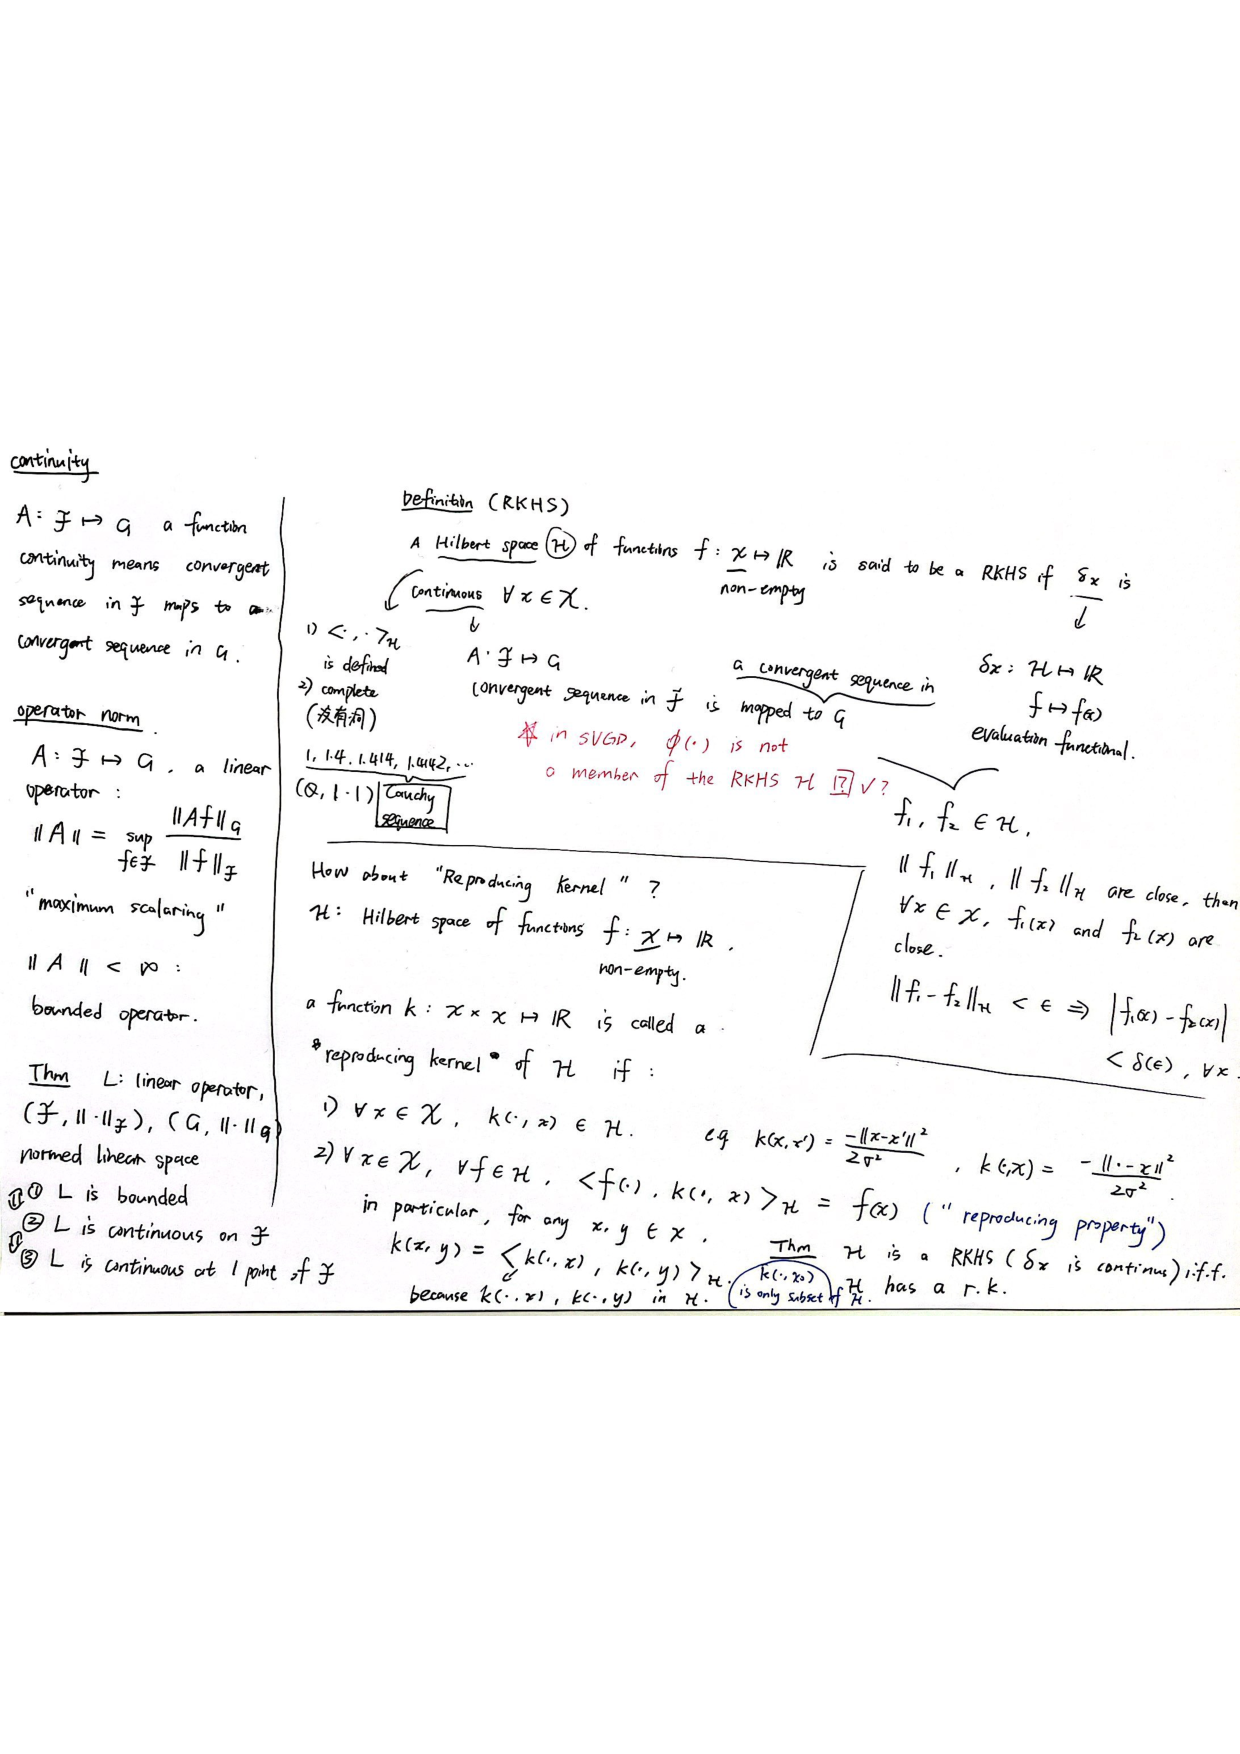
\includegraphics[width=18cm]{img/rkhs.pdf}
\section{Lemmas}
\begin{lemma}[First half of Lemma 2.3 of \citep{liu2016kernelized}] \label{lemma.1}
    Assume $p(\rvx)$ and $q(\rvx)$ are smooth densities supported on $\mathcal{X}$ and \textbf{scalar-valued} function $f(\rvx)$ is in the Stein class of $q$, we have:
    $$
    \E_{\rvx \sim q}\left[ \mathcal{A}_p f(\rvx) \right] = \E_{\rvx \sim q}\left[  (s_p(\rvx) - s_q(\rvx))f(\rvx)\right].
    $$
\end{lemma}

\begin{lemma}[Second half of Lemma 2.3 of \citep{liu2016kernelized}] \label{lemma.2}
    Assume $p(\rvx)$ and $q(\rvx)$ are smooth densities supported on $\mathcal{X}$ and when $\bm f(\rvx)$ is a $d \times 1$ \textbf{vector-valued} function in the Stein class of $q$, we have:
    $$
    \E_{\rvx \sim q}\left[ (s_p(\rvx) - s_q(\rvx))^\top \bm f(\rvx) \right] = \E_{\rvx \sim q}\left[ \trace\left( \mathcal{A}_p \bm f(\rvx) \right) \right].
    $$
\end{lemma}
\section{Introduction to measure theory}
\begin{itemize}
    \item Limit of a sequence: a sequence $x_1, x_2, \cdots, x_n$ is said to converge to $x$ or have limit if ...
    \item Cauchy sequence
    \item Algebraic structure
    \item measure space: $(\mathcal{X}, \mathcal{A}, \mu)$, where $\mathcal{X}$ is a set, $\mathcal{A}$ is a class of subsets of $\mathcal{X}$, and $\mu$ is a function that attach a nonnegative number to every set in $\mathcal{A}$.
    \item $\sigma$-algebra: $\mathcal{A}$ is call a $\sigma$-field of $\mathcal{X}$ if: 
    \begin{itemize}
        \item both $\emptyset$ and $\mathcal{X}$ in $\mathcal{A}$
        \item if $A$ in $\mathcal{A}$, then $A^c$ in $\mathcal{A}$ 
        \item if $A_1, \cdots, A_n$ is a countable collection of sets in $\mathcal{A}$, then both $\cup_i A_i$ and $\cap_i A_i$ in $\mathcal{A}$ 
    \end{itemize}
    \item measure: a function $\mu$  defined on $\mathcal{A}$ is called a (countably additive, nonnegative) measure if: (1)\quad (2)\quad (3)
    \item $(\Omega, \mathcal{F}, \mathbb{P})$ used to denote a probability space
    \item countable additive
    \item metric space, complete metric space, normed space
    \item inner product on a vector space
    \item Hilbert space: a vector space where inner product is defined, and contains all the limits of Cauchy sequences of functions
    \item kernel: $k: \mathcal{X} \times \mathcal{X} \to \mathbb{R}$ is a kernel if exists a $\mathbb{R}$-Hilbert space and a map $\phi: \mathcal{X} \to 
    \mathcal{H}$ s.t. $k(x, x') = \langle \phi(x), \phi(x') \rangle_{\mathcal{H}}, \forall x, x' \in \mathcal{X}$ 
\end{itemize}

\end{document}
